\documentclass[aspectratio=169, 14pt]{beamer}
\usepackage[utf8]{inputenc}
\usepackage{xeCJK}
\usepackage{graphicx}
\usepackage{transparent}
\usepackage[ruled, lined, linesnumbered, commentsnumbered]{algorithm2e}
\usepackage{pgfplots}
\usepackage{tikz}
\usetikzlibrary{matrix,backgrounds}
\usetikzlibrary{arrows}
\usetikzlibrary {arrows.meta}
\usetikzlibrary{calc,shadows.blur,fit,positioning}
\usetikzlibrary{decorations.pathreplacing}
\usetikzlibrary{shapes,snakes}
\usepackage{minted}
\usepackage{fontawesome5}
\usepackage{booktabs}
\usepackage{caption}
\usepackage{hyperref}
\hypersetup{
    colorlinks=true,
    linkcolor=blue,
    filecolor=magenta,      
    urlcolor=cyan,
    }
\urlstyle{same}
\usetheme{metropolis}
\metroset{block=fill}
\usecolortheme{default}
\definecolor{darkmidnightblue}{rgb}{0.0, 0.2, 0.4}
\definecolor{LightGray}{gray}{0.9}


%------------------------------------------------------------
%This block of code defines the information to appear in the
%Title page
\title[Database Principles and Applications] %optional
{数据库原理与应用}

\subtitle{SQL:空值和聚合查询}

\author[CHEN Zhongpu] % (optional)
{CHEN Zhongpu}

\institute[] % (optional)
{
  School of Computing and Artificial Intelligence \\
  \href{mailto:zpchen@swufe.edu.cn}{zpchen@swufe.edu.cn}
}

\date[] % (optional)
{SWUFE, Spring \the\year{}}

%End of title page configuration block
%------------------------------------------------------------


%------------------------------------------------------------
%The next block of commands puts the table of contents at the 
%beginning of each section and highlights the current section:

% \AtBeginSection[]
% {
%   \begin{frame}
%     \frametitle{Table of Contents}
%     \tableofcontents[currentsection]
%   \end{frame}
% }
%------------------------------------------------------------


\begin{document}

%The next statement creates the title page.
\frame{\titlepage}

%---------------------------------------------------------
%This block of code is for the table of contents after
%the title page
% \begin{frame}
% \frametitle{Table of Contents}
% \tableofcontents
% \end{frame}
%--------------------------------------------------------
\begin{frame}[fragile]
	\frametitle{复习}
	\begin{columns}
		\column{.4\textwidth}<1->
		\begin{enumerate}
			\item \texttt{create table}
			\item \texttt{select}, \texttt{from}, \texttt{where}
			\item \texttt{as}, \texttt{order by}
			\item 字符串、集合运算
		\end{enumerate}
		\column{.59\textwidth}<2->
		下面的 SQL 分别是什么含义?
		\begin{minted}[bgcolor=LightGray]{sql}
SELECT name FROM instructor 
WHERE dept_name <> 'Physics';

SELECT * FROM department
WHERE dept_name LIKE 'His%';
        \end{minted}
	\end{columns}

\end{frame}

{
% \usebackgroundtemplate{\transparent{0.3}{\begin{picture}
%     \includegraphics[height=0.7\paperheight]{cover}
% \end{picture}    
% }}
\usebackgroundtemplate{
	\tikz[overlay,remember picture]
	\node[opacity=0.3, at=(current page.south east),anchor=south east, yshift=2cm,xshift=4cm] {
		\includegraphics[height=0.6\paperheight]{cover}};
}
\begin{frame}
	\section{\textcolor{darkmidnightblue}{1. 空值}}
	\begin{quote}
		每种数据类型都可能包含一种特殊的值,叫做 \alert{null},表示一个缺失的值。
	\end{quote}
	\begin{tikzpicture}
		\node[fill=yellow,blur shadow={shadow xshift=-0.5ex},
			text width=20em,anchor=south west,rounded corners]
		{null有很多反直觉的行为,所以是学习的难点。};
	\end{tikzpicture}
\end{frame}

}

\begin{frame}
	\frametitle{1.1 空值与算术运算 }

	\begin{quote}
		如果算术表达式的任一输入为空,则算术表达式(如 \texttt{+ - * /})的结果为空。
	\end{quote}

	{\large \[r.A + 2\]}
\end{frame}

\begin{frame}
	\frametitle{人工插入数据}
	\begin{tikzpicture}
		\node at (0, 0) (insert){
			\includegraphics[width=.8\textwidth]{week5/insert}
		};
		\node[draw=red!80, very thick, rectangle, minimum size=0.8cm] at (0.6, -0.3){};
		\node[above=of insert, yshift=-1.2cm]{Step 1};

		\node[below=of insert, yshift=0.2cm] (zhongpu){
			\includegraphics[width=.8\textwidth]{week5/zhongpu}
		};
		\node[above=of zhongpu, yshift=-1.2cm]{Step 2};

		\node[below=of zhongpu, yshift=0.2cm] (submit){
			\includegraphics[width=.8\textwidth]{week5/insert}
		};
		\node[draw=red!80, very thick, rectangle, minimum size=0.8cm] at (3.2, -5.2){};
		\node[above=of submit, yshift=-1.2cm]{Step 3};

	\end{tikzpicture}

\end{frame}

\begin{frame}[fragile]
	\begin{minted}[bgcolor=LightGray]{sql}
-- 加 1000 元工资
SELECT 1000 + salary
FROM instructor
WHERE ID = '8888';
    \end{minted}

\end{frame}

\begin{frame}[fragile]
	\frametitle{1.2 空值的比较}
	{\large \faIcon{code}} 考虑 \texttt{1 > NULL},它的结果是什么?
	\begin{minted}[bgcolor=LightGray]{sql}
SELECT 1 > NULL;
    \end{minted}
	\pause
	布尔类型 (boolean):
	\begin{itemize}
		\item \texttt{true}
		\item \texttt{false}
		\item \texttt{unknown}
	\end{itemize}

	\begin{tikzpicture}
		\node[fill=yellow,blur shadow={shadow xshift=-0.5ex},
			text width=25em,anchor=south west,rounded corners]
		{\texttt{unknown} 是逻辑上的状态,在 SQL 中还是使用 \texttt{null} 来表示。所以 DataGrip 会将 \texttt{unknown} 显示为 \texttt{null}。};
	\end{tikzpicture}

\end{frame}

\begin{frame}[fragile]

	\begin{minted}[bgcolor=LightGray]{sql}
CREATE TABLE test1 (a boolean, b text);
    \end{minted}


	\includegraphics[width=.45\textwidth]{week5/boolean}
\end{frame}

\begin{frame}[fragile]
	\frametitle{练习 {\large \faIcon{code}} }
	Zhongpu 是否会在下面 SQL 的查询结果?

	\begin{minted}[bgcolor=LightGray]{sql}
SELECT * FROM instructor
WHERE salary < 80000;

SELECT * FROM instructor
WHERE salary >= 80000;
    \end{minted}
	\pause
	\begin{tikzpicture}
		\node[fill=yellow,blur shadow={shadow xshift=-0.5ex},
			text width=25em,anchor=south west,rounded corners]
		{\texttt{false} 和 \texttt{unknown} 的结果均不会出现在结果中。};
	\end{tikzpicture}

\end{frame}

\begin{frame}

	{\large \faIcon[regular]{lightbulb}} \textbf{思考}:当 \texttt{WHERE} 子句是 \texttt{NOT (salary < 80000)},Zhongpu 是否会出现?
	\pause
	\begin{itemize}
		\item \alert{AND}
		      \begin{itemize}
			      \item \texttt{true} \textbf{and} \texttt{unknown} is \texttt{unknown}
			      \item \texttt{false} \textbf{and} \texttt{unknown} is \texttt{false}
			      \item \texttt{unknown} \textbf{and} \texttt{unknown} is \texttt{unknown}
		      \end{itemize}
		\item \alert{OR}
		      \begin{itemize}
			      \item \texttt{true} \textbf{or} \texttt{unknown} is \texttt{true}
			      \item \texttt{false} \textbf{or} \texttt{unknown} is \texttt{unknown}
			      \item \texttt{unknown} \textbf{or} \texttt{unknown} is \texttt{unknown}
		      \end{itemize}
		\item \alert{NOT}
		      \begin{itemize}
			      \item \textbf{not} \texttt{unknown} is \texttt{unknown}
		      \end{itemize}
	\end{itemize}
\end{frame}

\begin{frame}[fragile]
	\frametitle{1.3 测试空值}
	\begin{tikzpicture}
		\node[fill=yellow,blur shadow={shadow xshift=-0.5ex},
			text width=25em,anchor=south west,rounded corners]
		{使用 \texttt{is null} 测试是否为空值。不能使用 \texttt{= != <>}。};
	\end{tikzpicture}

	\begin{minted}[bgcolor=LightGray]{sql}
-- 工资为 null
SELECT * FROM instructor WHERE salary IS NULL;

-- 工资不为 null
SELECT * FROM instructor WHERE salary IS NOT NULL;

-- (null = null) 的结果是 unknown
SELECT * FROM instructor WHERE salary = NULL;
    \end{minted}

\end{frame}

\begin{frame}[fragile]
	SQL 还支持使用 \alert{is unknown} 对布尔结果进行测试:

	\begin{minted}[bgcolor=LightGray]{sql}
/*
很多 DBMS 不支持 is unknown。
*/
SELECT * FROM instructor
WHERE (salary > 80000) IS UNKNOWN;

SELECT * FROM instructor
WHERE (salary > 80000) IS NOT UNKNOWN;
\end{minted}

\end{frame}

\begin{frame}[fragile]
	\frametitle{1.4 空值与 distinct}
	\begin{columns}
		\column{.3\textwidth}
		\begin{table}
			\begin{tabular}{ll}
				\toprule
				a     & b      \\
				\midrule
				true  & one    \\
				false & <null> \\
				true  & <null> \\
				\bottomrule
			\end{tabular}
		\end{table}
		\column{.69\textwidth}
		\begin{minted}[bgcolor=LightGray]{sql}
SELECT DISTINCT b FROM test1;
        \end{minted}
	\end{columns}

	\pause
	\texttt{select distinct} 子句能够消除重复结果。下面两种情况均视为相等:(1) 非空相等;(2) 都是 \texttt{null}。

\end{frame}

\begin{frame}[fragile]
	\frametitle{思考}

	通过实验结果猜测 \alert{coalesce} 函数的作用。

	\begin{minted}[bgcolor=LightGray]{sql}
SELECT name, coalesce(salary, 0)
FROM instructor;

SELECT a, coalesce(b, 'no content')
FROM test1;
\end{minted}

	\begin{quote}
		coalesce: If two or more things coalesce, they come or grow together to form one thing or system. 联合,合并
	\end{quote}

\end{frame}

\begin{frame}[fragile]
	\frametitle{练习 {\large \faIcon{code}} }
	使用 \texttt{case} 表达式重写下面的 SQL 语句:

	\begin{minted}[bgcolor=LightGray]{sql}
SELECT name, coalesce(salary, 0)
FROM instructor;
\end{minted}

	\pause
	\begin{minted}[bgcolor=LightGray, baselinestretch=1]{sql}
SELECT name,
       CASE
           WHEN salary is null THEN 0
           ELSE salary
       END
FROM instructor;
\end{minted}

\end{frame}

\begin{frame}
	\section{\textcolor{darkmidnightblue}{2. 聚集函数}}
	Aggregate functions: $x = f(X)$

	\begin{itemize}
		\item 最大值:$max$
		\item 最小值:$min$
		\item 平均值:$avg$
		\item 数量:$count$
		\item 和:$sum$
	\end{itemize}

\end{frame}

\begin{frame}[fragile]
	\frametitle{2.1 基本聚集}
	\begin{minted}[bgcolor=LightGray]{sql}
-- 计算机系的平均工资
SELECT avg(salary)
FROM instructor
WHERE dept_name = 'Comp. Sci.';
-- avg 和 sum 要求输入是数值类型
SELECT avg(salary) as avg_salary
FROM instructor
WHERE dept_name = 'Comp. Sci.';
-- 课程总数
SELECT count(*) FROM course;
\end{minted}
\end{frame}

\begin{frame}[fragile]
	聚集函数在计算时均忽略 \texttt{null},除了 \alert{count(*)}。
	\begin{minted}[bgcolor=LightGray]{sql}
SELECT avg(salary)
FROM instructor
WHERE dept_name = 'Comp. Sci.' 
  AND salary is not null;

-- count(*) 包括 null
SELECT count(*), count(salary) FROM instructor;
\end{minted}

	\begin{tikzpicture}
		\node[fill=yellow,blur shadow={shadow xshift=-0.5ex},
			text width=25em,anchor=south west,rounded corners]
		{仅 \texttt{count} 能与 \texttt{*} 连用;仅 \texttt{count(*)} 考虑 \texttt{null}。};
	\end{tikzpicture}

\end{frame}

\begin{frame}[fragile]
	在 2018 年 Spring 学期上课的老师总人数。

	\begin{minted}[bgcolor=LightGray]{sql}
SELECT count (DISTINCT ID)
FROM teaches
WHERE semester = 'Spring' AND year = 2018;
\end{minted}

	\begin{tikzpicture}
		\node[fill=yellow,blur shadow={shadow xshift=-0.5ex},
			text width=20em,anchor=south west,rounded corners]
		{\texttt{count (distinct *)} 是不合法的。};
	\end{tikzpicture}

\end{frame}

\begin{frame}[fragile]
	\frametitle{聚集:不能直接出现在 where}

	\begin{minted}[baselinestretch=1,bgcolor=LightGray]{sql}
-- 下面的查询是不合法的!
SELECT ID
FROM instructor
WHERE salary = min(salary);
    \end{minted}

	WHERE 子句中的谓词是在聚集之前起作用(it controls which rows go into the aggregate computation)。

\end{frame}

\begin{frame}[fragile]
	\frametitle{2.2 分组聚集}

	\begin{columns}
		\column{.54\textwidth}
		$x = f(X)$:从一个集合得到一个值

		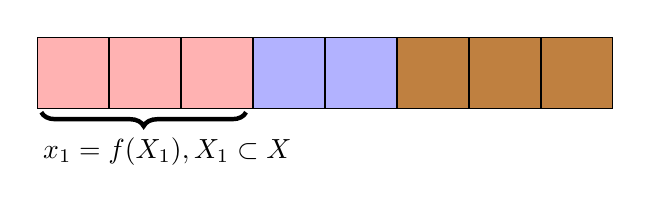
\begin{tikzpicture}[slot/.style={minimum size=0.9cm,rectangle}, data/.style={slot, fill=red!30}, data2/.style={slot, fill=blue!30}, data3/.style={slot, fill=brown}]
			\matrix [nodes=draw] (table)
			{
				\node[data] {};  &
				\node[data] {};  &
				\node[data] {};  &
				\node[data2] {}; &
				\node[data2] {}; &
				\node[data3] {}; &
				\node[data3] {}; &
				\node[data3] {};
				\\
			};
			\draw [decorate,
				decoration = {brace, mirror, amplitude=5pt}, ultra thick] (-3.6, -0.5) --  (-1, -0.5);

			\node at (-2, -1) {$x_1 = f(X_1), X_1 \subset X$};
		\end{tikzpicture}
		\column{.46\textwidth}
		\includegraphics[width=\textwidth]{week5/map}
		给定关系「成都市居民」,统计「温江区」的人口总数。
	\end{columns}

\end{frame}

\begin{frame}[fragile]
	\begin{columns}
		\column{.55\textwidth}
		SQL 中使用 \alert{group by} 实现按一个或多个属性进行分组。
		\column{.45\textwidth}
		\begin{figure}
			\includegraphics[width=\textwidth]{week5/group-salary}
			\caption*{\texttt{group by dept\_name}}
		\end{figure}
	\end{columns}
	\begin{minted}[baselinestretch=1,bgcolor=LightGray]{sql}
SELECT dept_name, avg(salary) as avg_salary
FROM instructor
GROUP BY dept_name;
\end{minted}
\end{frame}

\begin{frame}[fragile]

	找出每个系在2018年秋季学期有授课的教师人数。

	\begin{itemize}
		\item \texttt{instructor(ID, name, dept\_name, salary)}
		\item \texttt{teaches(ID, course\_id, sec\_id, semester, year)}
	\end{itemize}

	\begin{tikzpicture}
		\node[fill=yellow,blur shadow={shadow xshift=-0.5ex},
			text width=25em,anchor=south west,rounded corners]
		{按先 \texttt{from},再 \texttt{where},最后 \texttt{select} 的思路写复杂 SQL。};
	\end{tikzpicture}


	\begin{minted}[bgcolor=LightGray]{sql}
-- 第一步,先找到 2018 年秋有授课的教师和所在院系
SELECT dept_name, instructor.id
FROM instructor, teaches
WHERE instructor.id = teaches.id 
        AND semester = 'Spring' 
        AND year = 2018;
\end{minted}


\end{frame}

\begin{frame}[fragile]
	找出每个系在2018年秋季学期有授课的教师人数。

	\begin{itemize}
		\item \texttt{instructor(ID, name, dept\_name, salary)}
		\item \texttt{teaches(ID, course\_id, sec\_id, semester, year)}
	\end{itemize}

	\begin{tikzpicture}
		\node[fill=yellow,blur shadow={shadow xshift=-0.5ex},
			text width=25em,anchor=south west,rounded corners]
		{按先 \texttt{from},再 \texttt{where},最后 \texttt{select} 的思路写复杂 SQL。};
	\end{tikzpicture}

	\begin{minted}[bgcolor=LightGray, baselinestretch=1.1]{sql}
-- 第二步,再对院系分组并统计人数
SELECT dept_name, count (DISTINCT instructor.id)
FROM instructor, teaches
WHERE instructor.id = teaches.id 
        AND semester = 'Spring' 
        AND year = 2018
GROUP BY dept_name;
    \end{minted}
\end{frame}

\begin{frame}[fragile]
	\frametitle{练习 (1) {\large \faIcon{code}} }
	使用理论知识回答即可。
	\begin{columns}
		\column{.35\textwidth}
		\begin{verbatim}
=> SELECT * FROM test1;
x | y
---+---
a | 3
c | 2
b | 5
a | 1
(4 rows)    
    \end{verbatim}
		\column{.6\textwidth}

		下面 SQL 查询结果分别是?

		\begin{minted}[bgcolor=LightGray, baselinestretch=1.1]{sql} 
SELECT x FROM test1 GROUP BY x;   

SELECT x, sum(y) 
FROM test1 
GROUP BY x;
    \end{minted}

	\end{columns}
\end{frame}

\begin{frame}[fragile]
	\frametitle{练习 (2) {\large \faIcon{code}} }
	下面的查询是否合法?

	\begin{minted}[baselinestretch=1,bgcolor=LightGray]{sql}
SELECT dept_name, ID, avg(salary)
FROM instructor
GROUP BY dept_name;
\end{minted}

	\pause
	\begin{tikzpicture}
		\node[fill=yellow,blur shadow={shadow xshift=-0.5ex},
			text width=26em,anchor=south west,rounded corners]
		{重要提醒:出现在 \texttt{select} 子句中但没有被聚集的属性只能是出现在 \texttt{group by} 子句中的那些属性!};
	\end{tikzpicture}

\end{frame}

\begin{frame}[fragile]
	\frametitle{2.3 having 子句}
	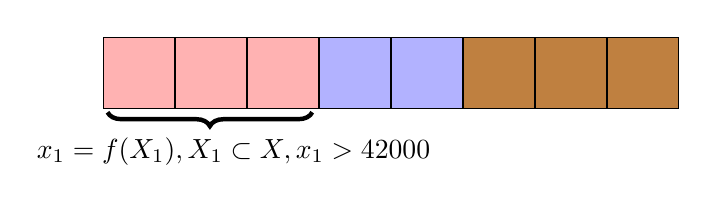
\begin{tikzpicture}[slot/.style={minimum size=0.9cm,rectangle}, data/.style={slot, fill=red!30}, data2/.style={slot, fill=blue!30}, data3/.style={slot, fill=brown}]
		\matrix [nodes=draw] (table)
		{
			\node[data] {};  &
			\node[data] {};  &
			\node[data] {};  &
			\node[data2] {}; &
			\node[data2] {}; &
			\node[data3] {}; &
			\node[data3] {}; &
			\node[data3] {};
			\\
		};
		\draw [decorate,
			decoration = {brace, mirror, amplitude=5pt}, ultra thick] (-3.6, -0.5) --  (-1, -0.5);

		\node at (-2, -1) {$x_1 = f(X_1), X_1 \subset X, x_1 > 42000$};
	\end{tikzpicture}

	如果需要\textbf{对分组限定条件},比如「平均工资超过 42000 元的系」,不能使用 \texttt{where} 子句,而需要使用 \texttt{having} 子句。
	\pause
	\begin{minted}[baselinestretch=1,bgcolor=LightGray]{sql}
SELECT dept_name, avg(salary) as avg_salary
FROM instructor
GROUP BY dept_name
HAVING avg(salary) > 42000;
    \end{minted}

\end{frame}

\begin{frame}[fragile]

	\begin{columns}
		\column{0.4\textwidth}
		{\large \faIcon[regular]{lightbulb}} 如何理解其执行次序?
		\begin{minted}[bgcolor=LightGray]{sql}
SELECT some_attr
FROM some_rel
WHERE where_cond
GROUP BY group_attr
HAVING having_cond;
        \end{minted}
		\column{.6\textwidth}
		\begin{enumerate}
			\item 最先根据 \texttt{from} 子句计算出一个关系
			\item 如果有 \texttt{where},将 \texttt{where} 的谓词应用到上述关系
			\item 如果有 \texttt{group by},在上述结果的基础上形成分组。如果没有,相当于整个元组集被当作一个分组
			\item 如果出现 \texttt{having},将应用到每个分组;不满足 \texttt{having} 的谓词的分组将被抛弃
			\item \texttt{select} 利用剩下的分组产生查询结果中的元组
		\end{enumerate}
	\end{columns}

\end{frame}

\begin{frame}[fragile]
	在 2017 年讲授的课程段,如果该课程段有至少 2 名学生选课,找出选修该课的所有学生的总学分的平均值。

	\begin{minted}[bgcolor=LightGray]{sql} 
SELECT course_id, semester, year, 
       sec_id, avg(tot_cred)
FROM student, takes
WHERE student.id = takes.id AND year = 2017
GROUP BY course_id, semester, year, sec_id
HAVING count(student.id) >= 2;
    \end{minted}

\end{frame}

\begin{frame}[fragile]
	\frametitle{练习 (1) {\large \faIcon{code}} }
	使用理论知识回答即可。

	\begin{columns}
		\column{.35\textwidth}
		\begin{verbatim}
=> SELECT * FROM test1;
x | y
---+---
a | 3
c | 2
b | 5
a | 1
(4 rows)    
    \end{verbatim}
		\column{.64\textwidth}

		下面 SQL 查询结果分别是?

		\begin{minted}[bgcolor=LightGray, baselinestretch=1.1]{sql} 
SELECT x, sum(y) FROM test1 
GROUP BY x HAVING sum(y) > 3;  

SELECT x, sum(y) FROM test1 
GROUP BY x HAVING x < 'c';
    \end{minted}

	\end{columns}
\end{frame}

\begin{frame}[fragile]
	\frametitle{练习 (2) {\large \faIcon{code}} }

	下面的 SQL 查询是否合法?

	\begin{minted}[bgcolor=LightGray, baselinestretch=1.1]{sql} 
SELECT x, sum(y) FROM test1 
GROUP BY x HAVING y > 3;  
\end{minted}

	\pause
	\begin{tikzpicture}
		\node[fill=yellow,blur shadow={shadow xshift=-0.5ex},
			text width=26em,anchor=south west,rounded corners]
		{重要提醒:出现在 \texttt{select} 和 \texttt{having} 子句中但没有被聚集的属性只能是出现在 \texttt{group by} 子句中的那些属性!};
	\end{tikzpicture}

\end{frame}


\begin{frame}[fragile]
	\frametitle{2.4 查询性能}
	\begin{minted}[bgcolor=LightGray, baselinestretch=1.1]{sql} 
-- 不推荐。having 子句一般使用聚集函数!
SELECT x, sum(y) FROM test1 
GROUP BY x 
HAVING x > 'a';

-- 性能更好
SELECT x, sum(y) FROM test1 
WHERE x > 'a'
GROUP BY x;
    \end{minted}



\end{frame}

\begin{frame}[fragile]
	\section{\textcolor{darkmidnightblue}{3. 嵌套子查询 (1)}}
	Nested sub-queries:\alert{select-from-where} 嵌套在另一个查询中

\end{frame}

\begin{frame}[fragile]
	\frametitle{3.1 from 子句中的子查询}
	任何 \texttt{select-from-where} 表达式返回的结果都是关系,因而可以被插入任何关系可以出现的位置。

	\begin{minted}[baselinestretch=1,bgcolor=LightGray]{sql}
SELECT dept_name, avg(salary) as avg_salary
FROM instructor
GROUP BY dept_name
HAVING avg(salary) > 42000;

/*
先得到一个子查询 (dept_name, avg_salary),
再对上述关系进行过滤。
*/
    \end{minted}

\end{frame}

\begin{frame}[fragile]

	\begin{minted}[baselinestretch=1,bgcolor=LightGray]{sql}
/*
先得到一个子查询 (dept_name, avg_salary),
再对上述关系进行过滤。

PG 要求对每个子查询结果关系都给一个名字,
即使该名字从不被引用。
*/
SELECT dept_name, avg_salary
FROM (SELECT dept_name, avg(salary) as avg_salary
      FROM instructor
      GROUP BY dept_name) AS a
WHERE avg_salary > 42000;
    \end{minted}

\end{frame}

\begin{frame}[fragile]
	\frametitle{3.2 集合成员资格 (set membership)}
	\begin{columns}
		\column{0.2\textwidth}
		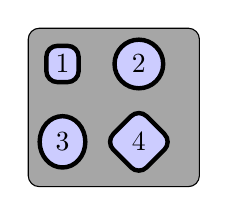
\begin{tikzpicture}
			\matrix[fill=gray!70,draw,rounded corners,nodes={draw, ultra thick, fill=blue!20},
				row sep=0.2cm,column sep=0.2cm] {
				\node[rectangle] {1}; &
				\node[circle] {2};      \\
				\node[ellipse] {3};   &
				\node[diamond] {4};   & \\
			};
		\end{tikzpicture}
		\column{0.8\textwidth}

		测试元组是否在集合 (enumerated set) 中,使用连接词 \texttt{in}。

		\begin{minted}[baselinestretch=1,bgcolor=LightGray]{sql}
-- 可以用 or 改写
SELECT DISTINCT name, salary
FROM instructor
WHERE name IN ('Mozart', 'Einstein');

SELECT DISTINCT name
FROM instructor
WHERE name NOT IN ('Mozart', 'Einstein');
    \end{minted}

	\end{columns}

\end{frame}

\begin{frame}[fragile]
	\texttt{in} 经常用于由 \texttt{select} 子句生成的集合中。

	\begin{minted}[baselinestretch=1,bgcolor=LightGray]{sql}
/*
找出所有同时在 2017 年 Fall 学期
和 2018年 Spring 学期开的课程。
*/
(SELECT course_id
FROM section
WHERE semester = 'Fall' AND year = 2017)
INTERSECT
(SELECT course_id
FROM section
WHERE semester = 'Spring' AND year = 2018);
\end{minted}

\end{frame}

\begin{frame}[fragile]

	\begin{columns}
		\column{0.3\textwidth}

		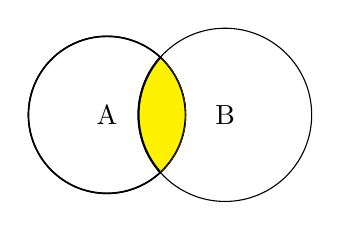
\begin{tikzpicture}[scale=0.5][thick]
			\begin{scope}
				\draw (0,0) circle (2cm);
				\draw (3,0) circle (2.2cm);
				\draw (0,0) node(2a) {A};
				\draw (3,0) node {B};
				\draw [clip](0,0) circle (2cm);
				\fill[yellow] (3,0) circle (2.2cm);
				\draw[black,thick] (0,0) circle(2cm);
				\draw[black,thick] (3,0) circle(2.2cm);
			\end{scope}
		\end{tikzpicture}
		\column{.7\textwidth}

		假设 2018 年 Spring 开设的课程号所构成的集合为 2018Spring,那么上述查询可以表述为:\textbf{查找所有 2017 年 Fall 开课的课程,看是否也是 2018Spring 集合中的成员。}
	\end{columns}

	\pause

	\begin{minted}[baselinestretch=1,bgcolor=LightGray]{sql}
SELECT DISTINCT course_id
FROM section
WHERE semester = 'Fall' AND year = 2017
    AND course_id IN (
        SELECT course_id
        FROM section
        WHERE semester = 'Spring' AND year = 2018
);
\end{minted}

\end{frame}

\begin{frame}[fragile]
	\frametitle{练习 {\large \faIcon{code}} }

	\begin{columns}
		\column{.3\textwidth}
		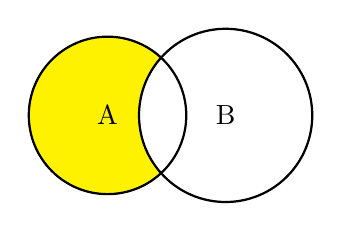
\begin{tikzpicture}[scale=0.5][thick]
			\begin{scope}
				\draw[fill=yellow] (0,0) circle (2cm);
				\draw[fill=white] (3,0) circle (2.2cm);
				\draw[black,thick] (0,0) circle(2cm);
				\draw[black,thick] (3,0) circle(2.2cm);
				\draw (0,0) node(3a) {A};
				\draw (3,0) node {B};
			\end{scope}
		\end{tikzpicture}
		\column{.7\textwidth}
		找出所有在 2017 年 Fall 学期,但不在 2018年 Spring 学期开的课程(使用 \texttt{in} 实现)。
	\end{columns}

\end{frame}

\begin{frame}[fragile]
	\frametitle{3.3 集合的比较}
	\begin{block}{Homework 2}
		请问下面的 SQL 语句的含义是什么?

		\begin{minted}[baselinestretch=1,bgcolor=LightGray]{sql}
SELECT DISTINCT T.name
FROM instructor AS T, instructor AS S
WHERE T.salary > S.salary AND S.dept_name = '会计';
\end{minted}
	\end{block}

	找出所有的老师,他们的工资比会计学院\alert{某一个}老师的工资高。
\end{frame}

\begin{frame}[fragile]
	「\textbf{至少比某一个要大}」在 SQL 中用 \texttt{> some} 表示。

	\begin{minted}[baselinestretch=1,bgcolor=LightGray]{sql}
SELECT name FROM instructor
WHERE salary > SOME(SELECT salary
                    FROM instructor
                    WHERE dept_name = 'History');

-- 也可表述为“大于最小值”
SELECT name FROM instructor
WHERE salary > (SELECT min(salary)
                FROM instructor
                WHERE dept_name = 'History');
\end{minted}

\end{frame}

\begin{frame}[fragile]
	\begin{tikzpicture}
		\node[fill=yellow,blur shadow={shadow xshift=-0.5ex},
			text width=26em,anchor=south west,rounded corners]
		{SQL 中 \texttt{any} 等价于 \texttt{some},
			但 \texttt{any} 在英语语义上有混淆,所以建议用 \texttt{some}。};
	\end{tikzpicture}
	\begin{columns}
		\column{0.25\textwidth}
		\begin{itemize}
			\item \texttt{< some}
			\item \texttt{<= some}
			\item \texttt{> some}
		\end{itemize}
		\column{0.25\textwidth}
		\begin{itemize}
			\item \texttt{>= some}
			\item \texttt{= some}
			\item \texttt{<> some}
		\end{itemize}
		\column{0.5\textwidth}
		注:\texttt{= some} 等价于 \texttt{in}。
	\end{columns}

\end{frame}

\begin{frame}[fragile]
	「\textbf{比所有要大}」在 SQL 中用 \texttt{> all} 表示。

	\begin{minted}[baselinestretch=1,bgcolor=LightGray]{sql}
SELECT name FROM instructor
WHERE salary > ALL(SELECT salary
                    FROM instructor
                    WHERE dept_name = 'History');
    \end{minted}
	\pause
	\begin{columns}
		\column{.2\textwidth}
		\begin{itemize}
			\item \texttt{< all}
			\item \texttt{<= all}
			\item \texttt{> all}
		\end{itemize}
		\column{.2\textwidth}
		\begin{itemize}
			\item \texttt{>= all}
			\item \texttt{= all}
			\item \texttt{<> all}
		\end{itemize}
		\column{.6\textwidth}
		\begin{tikzpicture}
			\node[fill=yellow,blur shadow={shadow xshift=-0.5ex},
				text width=12em,anchor=south west,rounded corners]
			{\texttt{<> all} 等价于 \texttt{not in}。};
		\end{tikzpicture}
	\end{columns}
\end{frame}

\begin{frame}[fragile]
	\frametitle{练习 {\large \faIcon{code}} }
	\begin{minted}[baselinestretch=1,bgcolor=LightGray]{sql}
SELECT dept_name FROM instructor
GROUP BY dept_name
HAVING avg(salary) >= ALL(SELECT avg(salary)
                           FROM instructor
                           GROUP BY dept_name);
    \end{minted}
	上面 SQL 查询的含义是什么?
\end{frame}

\begin{frame}
	\section{\textcolor{darkmidnightblue}{总结}}

	\begin{enumerate}
		\item \texttt{null} 值的处理
		\item 聚集函数、分组聚集
		\item \texttt{in, not in, > some, > all}
	\end{enumerate}
\end{frame}

\begin{frame}
	\frametitle{Homework 4}
	\href{https://github.com/ChenZhongPu/db-swufe/tree/master/05_sql}{05. SQL}

\end{frame}

\begin{frame}[fragile]
	\frametitle{SQL 查询:返回部分结果}

	\begin{minted}[baselinestretch=1,bgcolor=LightGray]{sql}
-- limit 不是标准语法,在 PG 和 MySQL 中支持
SELECT * FROM student LIMIT 5;
-- 如果 offset 值过大,查询会很低效
SELECT * FROM student LIMIT 5 OFFSET 2;
-- Oracle
SELECT * FROM student rownum <= 5;
-- SQLServer
SELECT TOP 5 * FROM student;

-- SQL 标准
SELECT * FROM student FETCH FIRST 5 ROWS ONLY;
    \end{minted}

\end{frame}

\begin{frame}[fragile]
	返回随机 N 条:

	\begin{minted}[baselinestretch=1,bgcolor=LightGray]{sql}
SELECT * 
FROM student 
ORDER BY random() LIMIT 5; 
\end{minted}

	请自行查阅文档,理解 \texttt{order by random()} 的含义。

\end{frame}

\begin{frame}
	\section{\textcolor{darkmidnightblue}{4. 嵌套子查询 (2)}}
	Nested sub-queries:\alert{select-from-where} 嵌套在另一个查询中

\end{frame}

\begin{frame}[fragile]
	\frametitle{4.1 标量子查询}
	标量子查询 (scalar sub-query) 只返回包含\textbf{单个属性的单个元组},能出现在 SQL 中的任意地方。

	\begin{minted}[baselinestretch=1,bgcolor=LightGray]{sql}

SELECT name FROM instructor
WHERE salary > (SELECT min(salary)
                FROM instructor
                WHERE dept_name = 'History');
\end{minted}

\end{frame}

\begin{frame}[fragile]
	列出每个学院及其对应的教师人数。

	\begin{minted}[baselinestretch=1,bgcolor=LightGray]{sql}
-- 请用 GROUP BY 重写
SELECT dept_name,
    (SELECT count(*)
    FROM instructor
    WHERE department.dept_name = instructor.dept_name)
    as num_instructor
FROM department;
 \end{minted}

	我们也能注意到可以在子查询的 \texttt{where} 子句中使用外层查询的 \alert{correlation name},此时该子查询被称为 \textbf{相关子查询} (correlated subquery)。

\end{frame}

\begin{frame}[fragile]
	\frametitle{4.2 空关系测试}
	使用 \alert{exists} 测试子查询返回的关系是否为空。

	\begin{minted}[baselinestretch=1,bgcolor=LightGray]{sql}
SELECT EXISTS(SELECT 1 FROM instructor);
\end{minted}

	\pause
	\textbf{例子}:找到修过ID为11011的老师的课程的学生总数。
	\begin{itemize}
		\item \texttt{\textbf{takes}(course\_id, sec\_id, semester, year, building, room\_number, time\_slot\_id)}
		\item \texttt{\textbf{teaches}(ID, course\_id, sec\_id, semester, year)}
	\end{itemize}
\end{frame}

\begin{frame}[fragile]

	\begin{minted}[bgcolor=LightGray]{sql}
/*
方法一:使用 in
*/
SELECT count(DISTINCT ID)
FROM takes
WHERE (course_id, sec_id, semester, year)
IN (SELECT course_id, sec_id, semester, year
    FROM teaches
    WHERE teaches.id = '10101');    
\end{minted}
\end{frame}

\begin{frame}[fragile]
	\begin{minted}[bgcolor=LightGray]{sql}
/*
方法二:使用 exists
*/
SELECT count(DISTINCT ID)
FROM takes
WHERE EXISTS(SELECT 1 FROM teaches
    WHERE teaches.id = '10101'
    AND takes.course_id = teaches.course_id
    AND takes.sec_id = teaches.sec_id
    AND takes.semester = teaches.semester
    AND takes.year = teaches.year);
    \end{minted}

\end{frame}

{\setbeamercolor{palette primary}{fg=black, bg=yellow}
\begin{frame}[standout]
	如果子查询的结果较多,建议使用 exists,而不是 in。
\end{frame}
}

\begin{frame}[fragile]
	\frametitle{练习}
	阅读课本 P.104,试用多表查询实现下面的嵌套查询。

	\begin{minted}[bgcolor=LightGray]{sql}
SELECT count(DISTINCT ID)
FROM takes
WHERE EXISTS(SELECT 1 FROM teaches
    WHERE teaches.id = '10101'
    AND takes.course_id = teaches.course_id
    AND takes.sec_id = teaches.sec_id
    AND takes.semester = teaches.semester
    AND takes.year = teaches.year);
    \end{minted}

\end{frame}

{\setbeamercolor{palette primary}{fg=black, bg=yellow}
\begin{frame}[standout]
	只要涉及多表,多表查询是万能的。
\end{frame}
}

\begin{frame}[fragile]
	\frametitle{4.3 with 子句}

	\alert{with} 字句定义了一个临时的关系,用于当前查询。

	\begin{minted}[bgcolor=LightGray]{sql}
WITH max_buedget(value) AS
    (SELECT max(budget)
     FROM department)
SELECT budget
FROM department, max_buedget
WHERE department.budget = max_buedget.value;
\end{minted}
\end{frame}

\begin{frame}[fragile]

	\begin{minted}[bgcolor=LightGray]{sql}
-- 列出所有工资总额大于所有系平均工资总额的系
WITH dept_total (dept_name, value) AS
    (SELECT dept_name, sum(salary)
     FROM instructor
     GROUP BY dept_name),
    dept_total_avg(value) AS
    (SELECT avg(value)
     FROM dept_total)
SELECT dept_name
FROM dept_total, dept_total_avg
WHERE dept_total.value > dept_total_avg.value;
\end{minted}

\end{frame}

\begin{frame}[fragile]
	\begin{minted}[bgcolor=LightGray]{sql}
-- 如果不使用 with 子句
SELECT dept_name
FROM instructor
GROUP BY dept_name
HAVING sum(salary) > (SELECT avg(value)
                        FROM (SELECT sum(salary)
                            FROM instructor
                            GROUP BY dept_name)
                        AS sum_salary(value));
                        \end{minted}
\end{frame}

\begin{frame}[fragile]
	\frametitle{练习 {\large \faIcon{code}} }
	\begin{minted}[bgcolor=LightGray, baselinestretch=1]{sql}
CASE
    WHEN condition1 THEN result1
    WHEN condition2 THEN result2
    WHEN conditionN THEN resultN
    ELSE result
END;
    \end{minted}

	考虑关系模式 marks(ID, score),并规定如果 score < 60 等级为 C,60 $\leq$ score < 80 等级为 B,score $\geq$ 80 等级为 A。

	\textbf{问题}:显示不同成绩等级的学生总数。

\end{frame}

\begin{frame}[fragile]

	\begin{minted}[bgcolor=LightGray]{sql}
WITH grades AS (
    SELECT ID,
        CASE
            WHEN score < 60 THEN 'C'
            WHEN score >= 80 THEN 'A'
            ELSE 'B'
        END AS grade
    FROM marks
)
SELECT grade, count(ID)
FROM grades
GROUP BY grade;
    \end{minted}

\end{frame}

\end{document}
